\documentclass{article}
\usepackage[utf8]{inputenc}
\usepackage{graphicx}
\usepackage[spanish]{babel}
\usepackage{siunitx}
\usepackage{float}
\setlength\parindent{0pt}
\tolerance=9999
\hyphenpenalty=10000
\exhyphenpenalty=100
\graphicspath{ {./images/} }

\title{Aproximación de la Aceleración Gravitacional en la Tierra}
\author{Matias Vicente, Guillermo Wajner et al.}
\date{16 de mayo de 2022}

\begin{document}

\maketitle

\section{Introducci\'{o}n}

En el presente informe de pr\'{a}ctica de laboratorio se buscar\'{a} determinar una aproximación de la aceleración gravitacional a trav\'{e}z de datos extra\'{i}dos de un experimento realizado en clase por los participantes en cuesti\'{o}n.

\section{Objetivo}

Determinar una aproximación del valor de la aceleraci\'{o}n gravitacional en el laboratorio. 

\section{Marco Te\'{o}rico}

El movimiento descrito por un objeto solo influenciado por la fuerza gravitatoria es llamado movimiento de ca\'{i}da libre. Este es un caso espec\'{i}fico de movimiento rectil\'{i}neo uniformemente variado (MRUV). La ecuaci\'{o}n que relaciona el desplazamiento ($\Delta x$), la aceleraci\'{o}n gravitatoria ($g$), la velocidad inicial ($v_0$) y el tiempo de un MRUV es la siguiente: 

\begin{equation}
\Delta x=tv_0+\frac{gt^2}{2}
\end{equation}

Esta ecuaci\'{o}n puede ser reescrita para $g$ de la siguiente manera:

\begin{equation}
\label{eqn:g}
g=\frac{2\Delta x-tv_0}{t^2}
\end{equation}

Para facilitar el experimento, no fue tomada en cuenta la fuerza de rozamiento, ya que su efecto es despreciable en esta situaci\'{o}n.

\section{Procedimiento}

Para realizar el experimento, fue decidido dejar caer una goma de borrar desde una altura determinada y controlar el tiempo que tarda la misma en tocar el suelo. La altura escogida ($\Delta x$) fue $1,928m$ medidos con una regla T en la pared del laboratorio, donde se hizo una marca con l\'{a}piz. Desde esta marca ser\'{i}a dejada caer la goma reiteradas veces. Para tomar la medida del tiempo, uno de los participantes del experimento fue encargado de controlar el cron\'{o}metro, deteniéndolo cuando la goma alcanza el suelo, y el otro participante fue encargado en dejar la goma caer al comenzar el cron\'{o}metro.

\section{Datos Obtenidos}

El procedimiento descrito fue repetido 200 veces registrando el valor de $t$ obtenido en segundos, de los cuales los 100 valores mas cercanos a la media fueron tomados. El cuadro \ref{table:tvalues} a continuaci\'{o}n contiene los valores de $t$ utilizados.

\begin{table}[h]
\centering
\begin{tabular}{llllllllll}
0.55 & 0.58 & 0.59 & 0.61 & 0.62 & 0.63 & 0.63 & 0.65 & 0.66 & 0.68  \\
0.56 & 0.58 & 0.59 & 0.61 & 0.62 & 0.63 & 0.63 & 0.65 & 0.66 & 0.69  \\
0.56 & 0.58 & 0.59 & 0.61 & 0.62 & 0.63 & 0.64 & 0.65 & 0.68 & 0.69  \\
0.56 & 0.58 & 0.59 & 0.61 & 0.62 & 0.63 & 0.64 & 0.65 & 0.68 & 0.69  \\
0.57 & 0.58 & 0.59 & 0.61 & 0.62 & 0.63 & 0.64 & 0.65 & 0.68 & 0.70   \\
0.57 & 0.58 & 0.59 & 0.61 & 0.62 & 0.63 & 0.64 & 0.66 & 0.68 & 0.70   \\
0.57 & 0.58 & 0.59 & 0.61 & 0.62 & 0.63 & 0.64 & 0.66 & 0.68 & 0.70   \\
0.58 & 0.58 & 0.60 & 0.61 & 0.62 & 0.63 & 0.64 & 0.66 & 0.68 & 0.71  \\
0.58 & 0.59 & 0.60 & 0.61 & 0.62 & 0.63 & 0.64 & 0.66 & 0.68 & 0.72  \\
0.58 & 0.59 & 0.60 & 0.61 & 0.62 & 0.63 & 0.65 & 0.66 & 0.68 & 0.72 
\end{tabular}
\caption{valores de $t$ utilizados}
\label{table:tvalues}
\end{table}

\pagebreak

\section{Procesamiento de Datos}

Los valores del cuadro \ref{table:tvalues} fueron insertados en la ecuaci\'{o}n (\ref{eqn:g}), y la distribuci\'{o}n de los resultados de esto fue analizada. En la figura \ref{figure:distg} se presenta un gr\'{a}fico de frecuencia para los valores de $g$ en intervalos de \qty[mode = text]{0.60}{m/s^{2}}.

\begin{figure}[H]
\centering
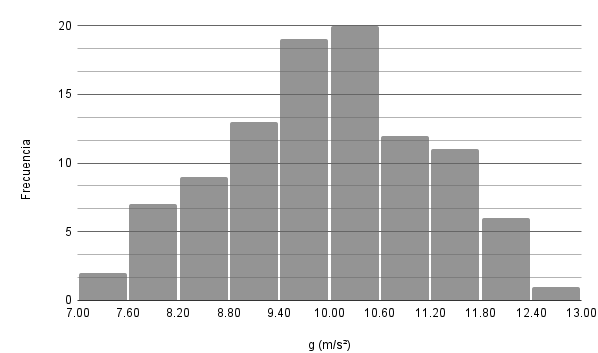
\includegraphics[width=\textwidth]{images/chart1.png}
\caption{distribuci\'{o}n de valores de $g$}
\label{figure:distg}
\end{figure}

En este gr\'{a}fico es posible observar que la distribuci\'{o}n de los valores se asemeja a una distibuci\'{o}n gaussiana.
\\
\\
Posteriormente, los valores de $g$ obtenidos fueron tambi\'{e}n promediados, resultando en un valor $\bar{g}=\qty[mode = text] {9.917868402} {m/s^{2}}$.

\section{Conclusi\'{o}n}

Ya con nuestra aproximación de la aceleración gravitatoria obtenida la podemos comparar con el valor estándar de $g$, , que es cercano al valor est\'{a}ndar de $g$, \qty[mode = text] {9.80665} {m/s^{2}}. Al comparar los valores encontramos que $\Delta g\approx \qty[mode = text]{0.1}{m/s^{2}}$, variaci\'{o}n atribuible a errores experimentales. Teniendo en cuenta esto, podemos considerar que el experimento fue relativamente exitoso, sin embargo, es posible implementar mejores m\'{e}todos para mejorar la presici\'{o}n de la aproximaci\'{o}n.

\end{document}
